% This file was created with tikzplotlib v0.10.1.
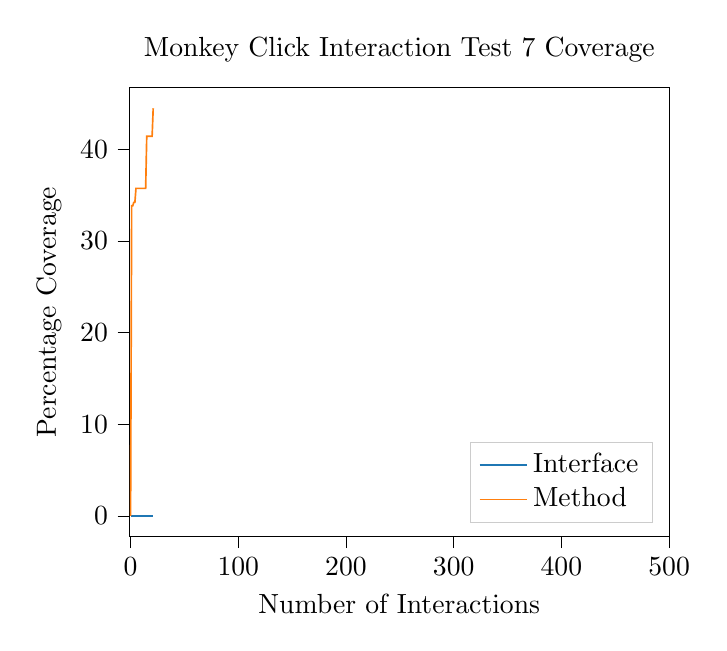
\begin{tikzpicture}

\definecolor{darkgray176}{RGB}{176,176,176}
\definecolor{darkorange25512714}{RGB}{255,127,14}
\definecolor{lightgray204}{RGB}{204,204,204}
\definecolor{steelblue31119180}{RGB}{31,119,180}

\begin{axis}[
legend cell align={left},
legend style={
  fill opacity=0.8,
  draw opacity=1,
  text opacity=1,
  at={(0.97,0.03)},
  anchor=south east,
  draw=lightgray204
},
tick align=outside,
tick pos=left,
title={Monkey Click Interaction Test 7 Coverage},
x grid style={darkgray176},
xlabel={Number of Interactions},
xmin=-1.05, xmax=500,
xtick style={color=black},
y grid style={darkgray176},
ylabel={Percentage Coverage},
ymin=-2.2245, ymax=46.7145,
ytick style={color=black}
]
\addplot [semithick, steelblue31119180]
table {%
0 0
1 0
2 0
3 0
4 0
5 0
6 0
7 0
8 0
9 0
10 0
11 0
12 0
13 0
14 0
15 0
16 0
17 0
18 0
19 0
20 0
21 0
};
\addlegendentry{Interface}
\addplot [semithick, darkorange25512714]
table {%
0 0
1 33.84
2 33.84
3 34.22
4 34.22
5 35.74
6 35.74
7 35.74
8 35.74
9 35.74
10 35.74
11 35.74
12 35.74
13 35.74
14 35.74
15 41.44
16 41.44
17 41.44
18 41.44
19 41.44
20 41.44
21 44.49
};
\addlegendentry{Method}
\end{axis}

\end{tikzpicture}
